This section expands upon the motivation for programming languages to contain a memory model and introduces a few core concepts that parallel programmers should familiarize themselves with:\par

\begin{itemize}
	\item Data races and synchronization
	\item Barriers and fences
	\item Atomic operations
	\item Memory ordering
\end{itemize}

Understanding these concepts at a high level is necessary to appreciate their expression and usage in C++, SYCL, and DPC++. Readers with extensive experience in parallel programming, especially using C++, may wish to skip ahead.\par

\hspace*{\fill} \par %插入空行
\textbf{Data Races and Synchronization}

The operations that we write in our programs typically do not map directly to a single hardware instruction or micro-operation. A simple addition operation such as data[i] += x may be broken down into a sequence of several instructions or micro-operations:\par

\begin{enumerate}
	\item Load data[i] from memory into a temporary 	(register).
	\item Compute the result of adding x to data[i].
	\item Store the result back to data[i].
\end{enumerate}

This is not something that we need to worry about when developing sequential applications—the three stages of the addition will be executed in the order that we expect, as depicted in Figure 19-1.\par

\hspace*{\fill} \par %插入空行
Figure 19-1. Sequential execution of data[i] += x broken into three separate operations
\begin{center}
	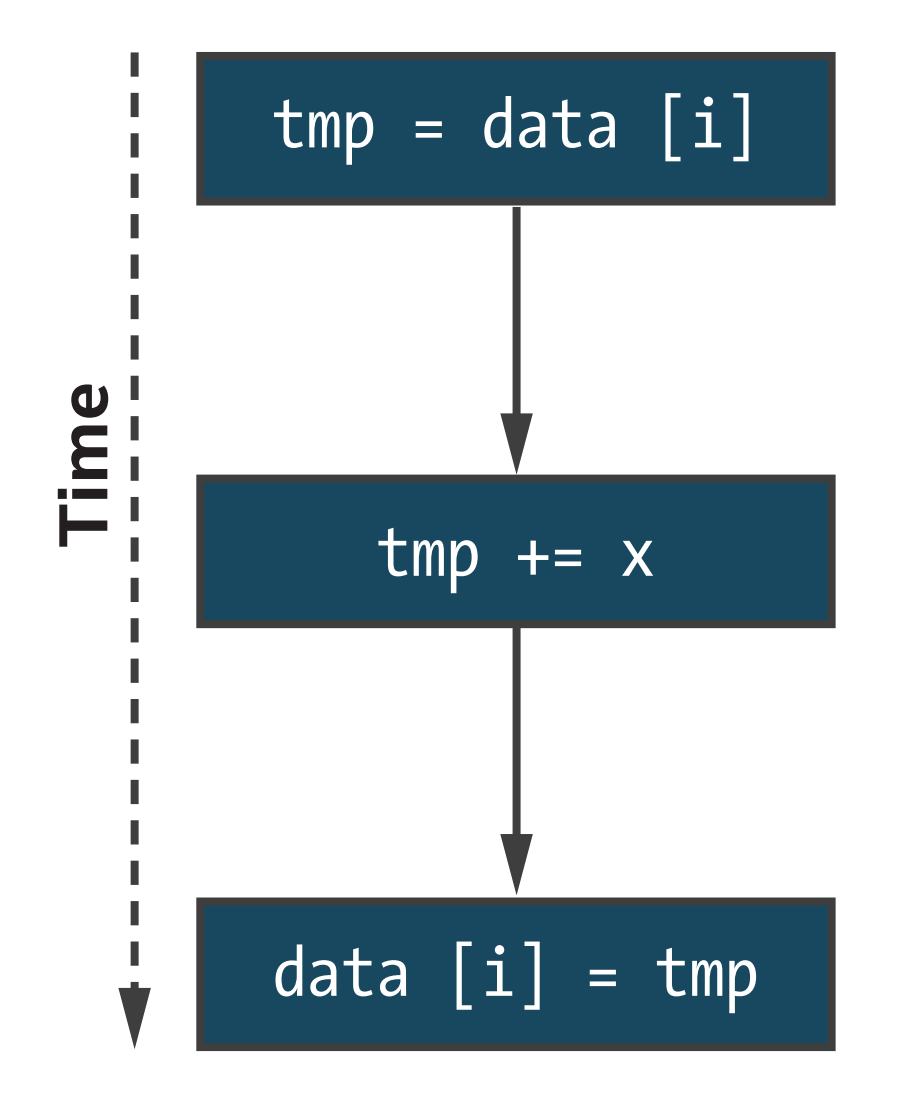
\includegraphics[width=1.0\textwidth]{content/chapter-19/images/2}
\end{center}

Switching to parallel application development introduces an extra level of complexity: if we have multiple operations being applied to the same data concurrently, how can we be certain that their view of that data is consistent? Consider the situation shown in Figure 19-2, where two executions of data[i] += x have been interleaved. If the two executions use different values of i, the application will execute correctly. If they use the same value of i, both load the same value from memory, and one of the results is overwritten by the other! This is just one of many possible ways in which their operations could be scheduled, and the behavior of our application depends on which program instance gets to which data first—our application contains a data race.\par

\hspace*{\fill} \par %插入空行
Figure 19-2. One possible interleaving of data[i] += x executed 
concurrently
\begin{center}
	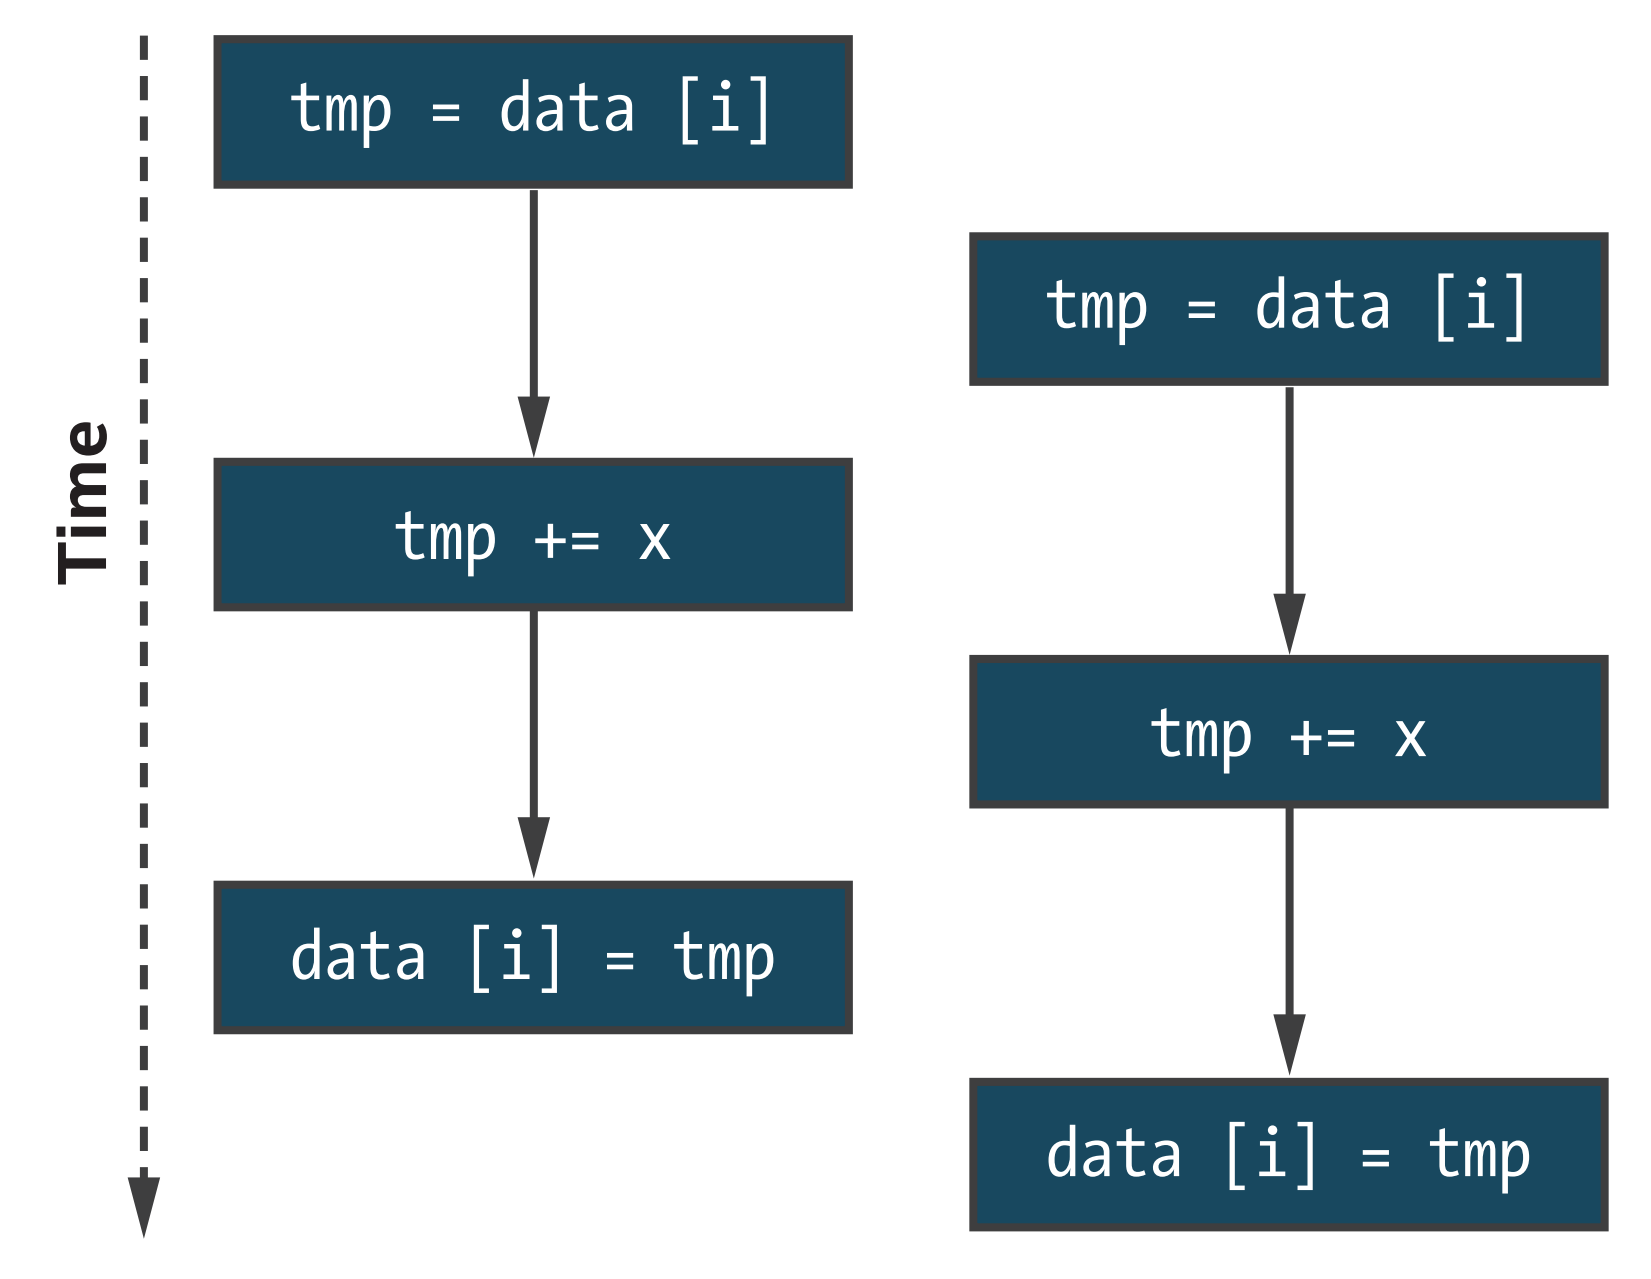
\includegraphics[width=1.0\textwidth]{content/chapter-19/images/3}
\end{center}

The code in Figure 19-3 and its output in Figure 19-4 show how easily this can happen in practice. If M is greater than or equal to N, the value of j in each program instance is unique; if it isn’t, values of j will conflict, and updates may be lost. We say may be lost because a program containing a data race could still produce the correct answer some or all of the time (depending on how work is scheduled by the implementation and hardware). Neither the compiler nor the hardware can possibly know what this program is intended to do or what the values of N and M may be at runtime—it is our responsibility as programmers to understand whether our programs may contain data races and whether they are sensitive to execution order.\par

\hspace*{\fill} \par %插入空行
Figure 19-3. Kernel containing a data race
\begin{lstlisting}[caption={}]
int* data = malloc_shared<int>(N, Q);
std::fill(data, data + N, 0);

Q.parallel_for(N, [=](id<1> i) {
	int j = i % M;
	data[j] += 1;
}).wait();

for (int i = 0; i < N; ++i) {
	std::cout << "data [" << i << "] = " << data[i] << "\n";
}
\end{lstlisting}

\hspace*{\fill} \par %插入空行
Figure 19-4. Sample output of the code in Figure 19-3 for small values of N and M
\begin{tcolorbox}[colback=white,colframe=black]
N = 2, M = 2:\\
data [0] = 1\\
data [1] = 1\\
\\
N = 2, M = 1:\\
data [0] = 1\\
data [1] = 0
\end{tcolorbox}

In general, when developing massively parallel applications, we should not concern ourselves with the exact order in which individual workitems execute—there are hopefully hundreds (or thousands!) of workitems executing concurrently, and trying to impose a specific ordering upon them will negatively impact both scalability and performance. Rather, our focus should be on developing portable applications that execute correctly, which we can achieve by providing the compiler (and hardware) with information about when program instances share data, what guarantees are needed when sharing occurs, and which execution orderings are legal.\par

\begin{tcolorbox}[colback=red!5!white,colframe=red!75!black]
Massively parallel applications should not be concerned with the exact order in which individual work-items execute!
\end{tcolorbox}

\hspace*{\fill} \par %插入空行
\textbf{Barriers and Fences}

One way to prevent data races between work-items in the same group is to introduce synchronization across different program instances using workgroup barriers and appropriate memory fences. We could use a work-group barrier to order our updates of data[i] as shown in Figure 19-5, and an updated version of our example kernel is given in Figure 19-6. Note that because a work-group barrier does not synchronize work-items in different groups, our simple example is only guaranteed to execute correctly if we limit ourselves to a single work-group!\par

\hspace*{\fill} \par %插入空行
Figure 19-5. Two instances of data[i] += x separated by a barrier
\begin{center}
	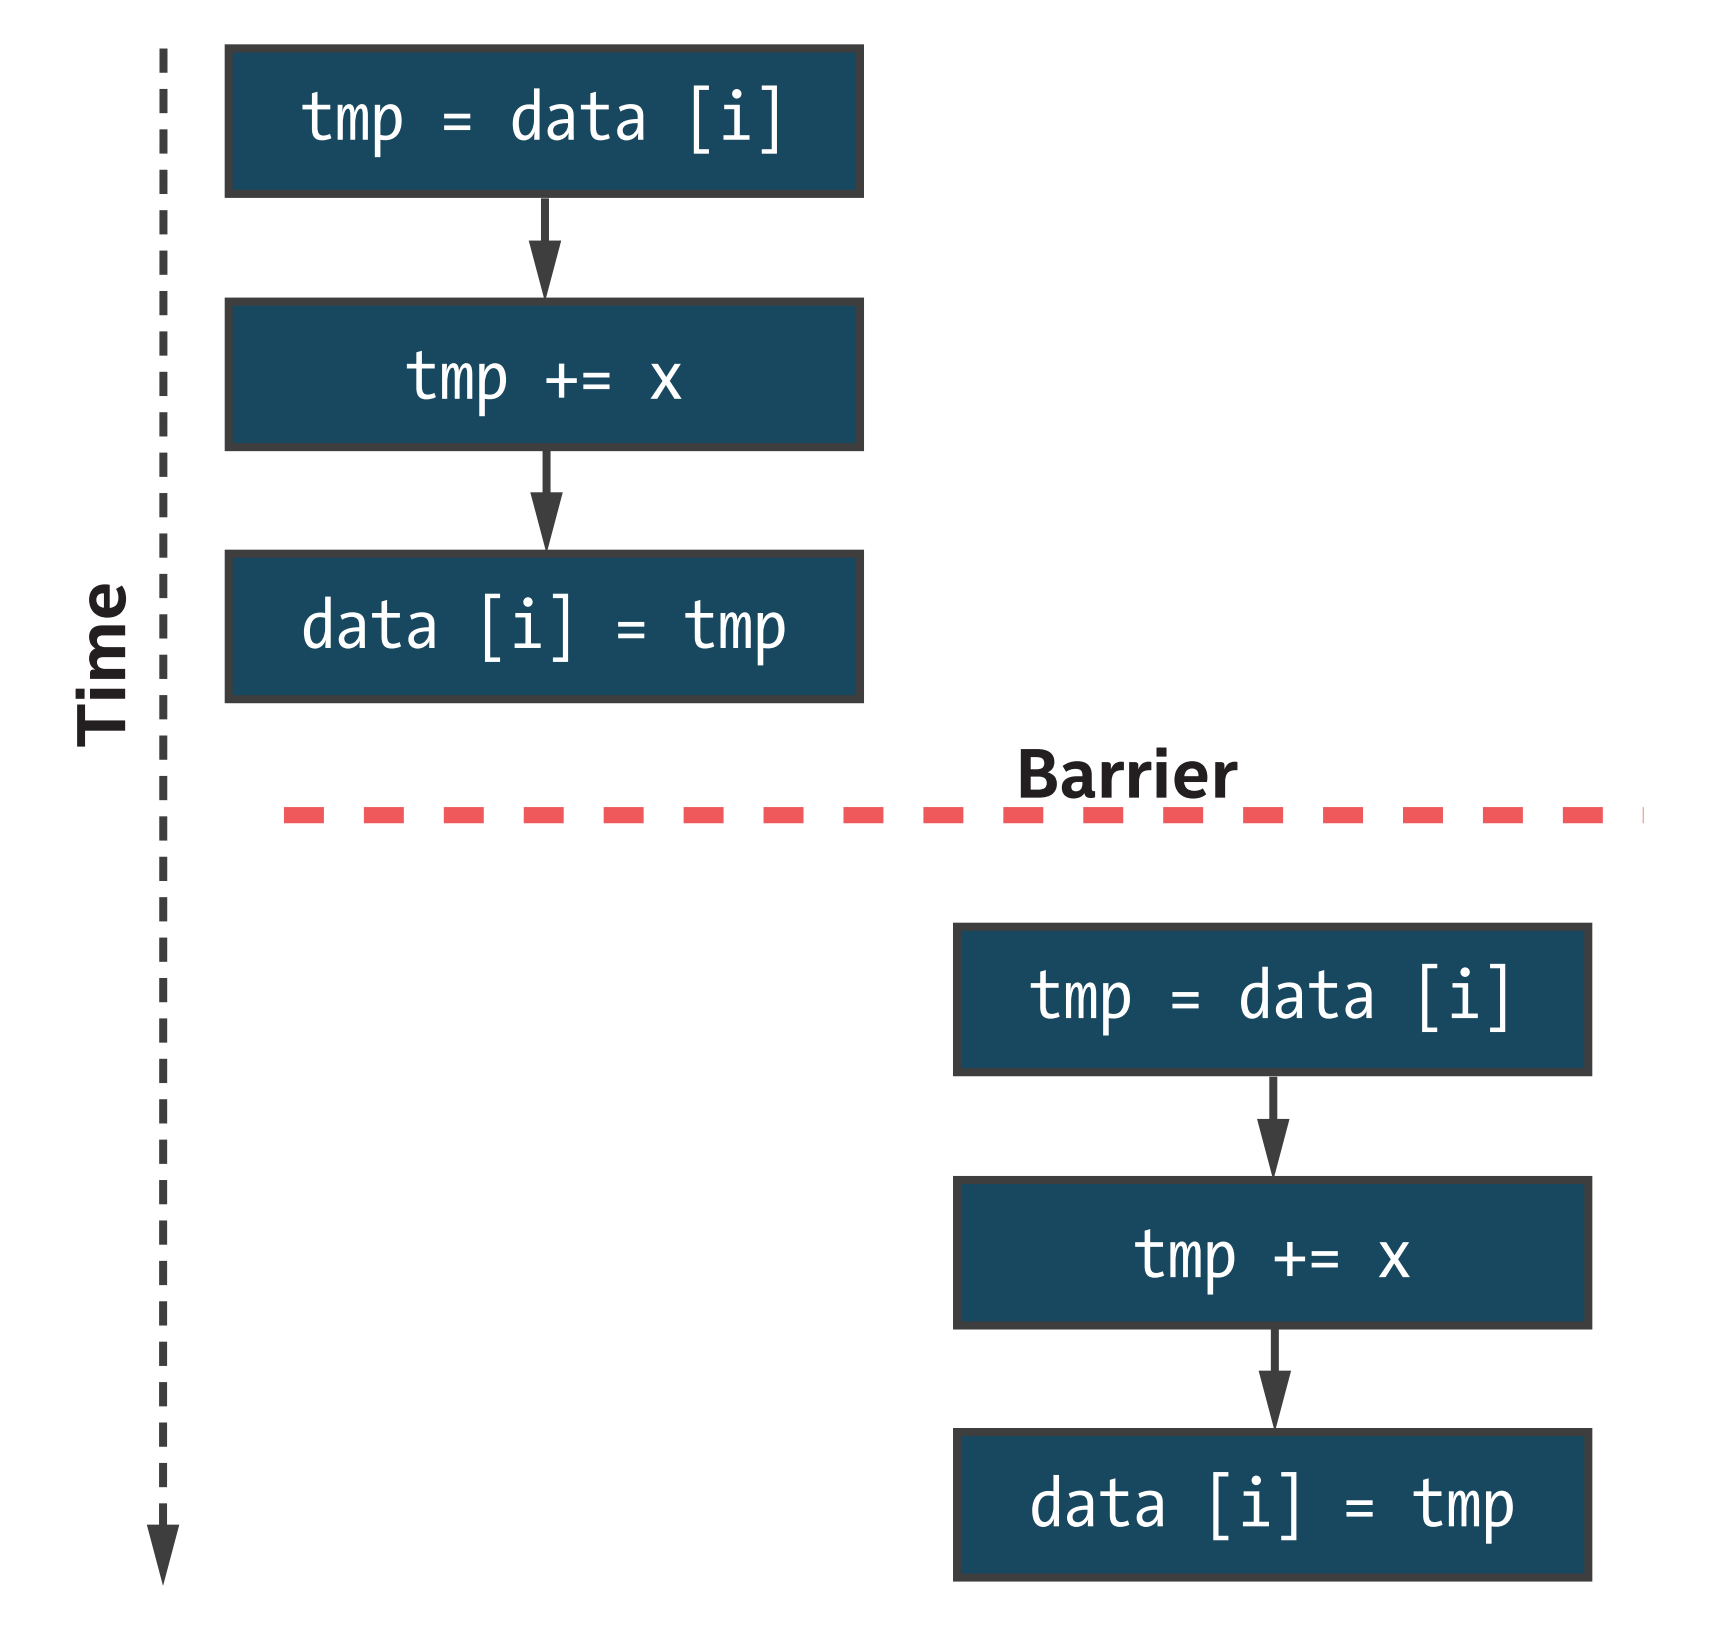
\includegraphics[width=1.0\textwidth]{content/chapter-19/images/4}
\end{center}

\hspace*{\fill} \par %插入空行
Figure 19-6. Avoiding a data race using a barrier
\begin{lstlisting}[caption={}]
int* data = malloc_shared<int>(N, Q);
std::fill(data, data + N, 0);

// Launch exactly one work-group
// Number of work-groups = global / local
range<1> global{N};
range<1> local{N};

Q.parallel_for(nd_range<1>{global, local}, [=](nd_item<1> it) {
	int i = it.get_global_id(0);
	int j = i % M;
	for (int round = 0; round < N; ++round) {
		// Allow exactly one work-item update per round
		if (i == round) {
			data[j] += 1;
		}
		it.barrier();
	}
}).wait();

for (int i = 0; i < N; ++i) {
	std::cout << "data [" << i << "] = " << data[i] << "\n";
}
\end{lstlisting}

Although using a barrier to implement this pattern is possible, it is not typically encouraged—it forces the work-items in a group to execute sequentially and in a specific order, which may lead to long periods of inactivity in the presence of load imbalance. It may also introduce more synchronization than is strictly necessary—if the different program instances happen to use different values of i, they will still be forced to synchronize at the barrier.\par

Barrier synchronization is a useful tool for ensuring that all work-items in a work-group or sub-group complete some stage of a kernel before proceeding to the next stage, but is too heavy-handed for fine-grained (and potentially data-dependent) synchronization. For more general synchronization patterns, we must look to atomic operations.\par

\hspace*{\fill} \par %插入空行
\textbf{Atomic Operations}

Atomic operations enable concurrent access to a memory location without introducing a data race. When multiple atomic operations access the same memory, they are guaranteed not to overlap. Note that this guarantee does not apply if only some of the accesses use atomics and that it is our responsibility as programmers to ensure that we do not concurrently access the same data using operations with different atomicity guarantees.\par

\begin{tcolorbox}[colback=red!5!white,colframe=red!75!black]
Mixing atomic and non-atomic operations on the same memory location(s) at the same time results in undefined behavior!
\end{tcolorbox}

If our simple addition is expressed using atomic operations, the result may look like Figure 19-8—each update is now an indivisible chunk of work, and our application will always produce the correct result. The corresponding code is shown in Figure 19-7—we will revisit the atomic\_ref class and the meaning of its template arguments later in the chapter.\par

\hspace*{\fill} \par %插入空行
Figure 19-7. Avoiding a data race using atomic operations
\begin{lstlisting}[caption={}]
int* data = malloc_shared<int>(N, Q);
std::fill(data, data + N, 0);

Q.parallel_for(N, [=](id<1> i) {
	int j = i % M;
	atomic_ref<int, memory_order::relaxed, memory_scope::system,
			   access::address_space::global_space> atomic_data(data[j]);
	atomic_data += 1;
}).wait();

for (int i = 0; i < N; ++i) {
	std::cout << "data [" << i << "] = " << data[i] << "\n";
}
\end{lstlisting}

\hspace*{\fill} \par %插入空行
Figure 19-8. An interleaving of data[i] += x executed concurrently with atomic operations
\begin{center}
	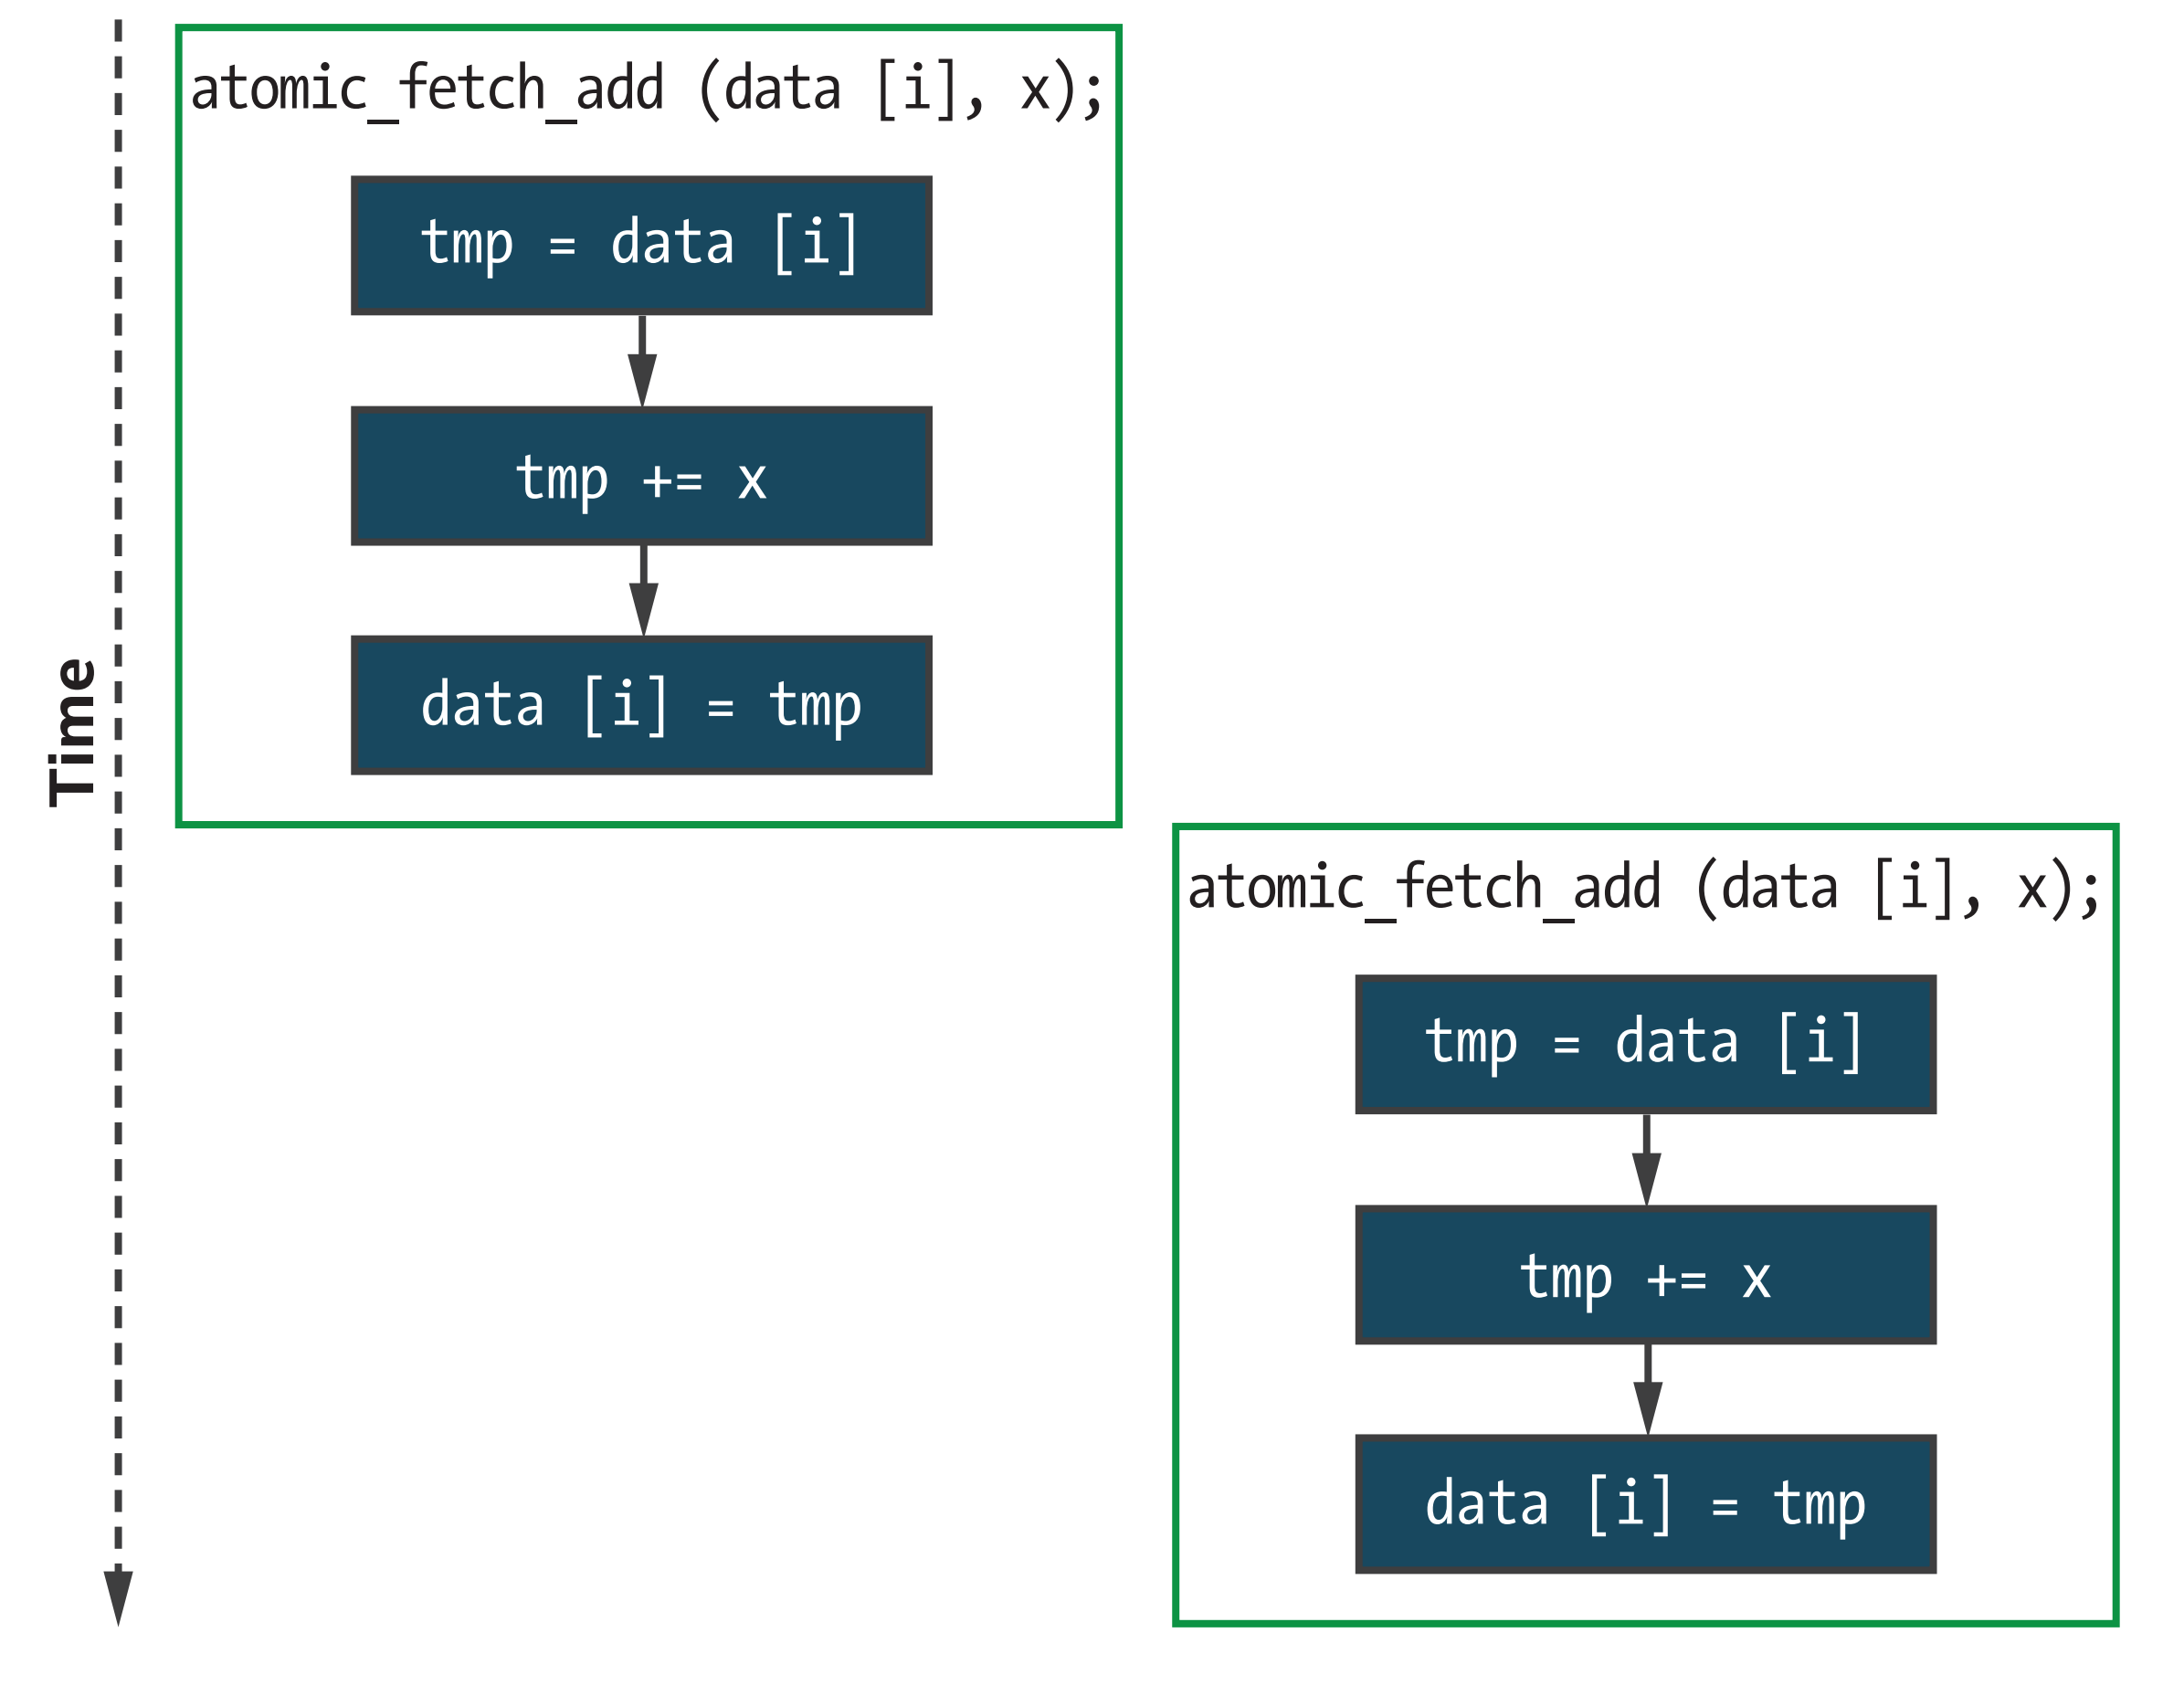
\includegraphics[width=1.0\textwidth]{content/chapter-19/images/5}
\end{center}

However, it is important to note that this is still only one possible execution order. Using atomic operations guarantees that the two updates do not overlap (if both instances use the same value of i), but there is still no guarantee as to which of the two instances will execute first. Even more importantly, there are no guarantees about how these atomic operations are ordered with respect to any non-atomic operations in different program instances.\par

\hspace*{\fill} \par %插入空行
\textbf{Memory Ordering}

Even within a sequential application, optimizing compilers and the hardware are free to re-order operations if they do not change the observable behavior of an application. In other words, the application must behave as if it ran exactly as it was written by the programmer.\par

Unfortunately, this as-if guarantee is not strong enough to help us reason about the execution of parallel programs. We now have two sources of re-ordering to worry about: the compiler and hardware may re-order the execution of statements within each sequential program instance, and the program instances themselves may be executed in any (possibly interleaved) order. In order to design and implement safe communication protocols between program instances, we need to be able to constrain this re-ordering. By providing the compiler with information about our desired memory order, we can prevent re-ordering optimizations that are incompatible with the intended behavior of our applications.\par

Three commonly available memory orderings are\par

\begin{enumerate}
	\item A relaxed memory ordering
	\item An acquire-release or release-acquire memory ordering
	\item A sequentially consistent memory ordering
\end{enumerate}

Under a relaxed memory ordering, memory operations can be reordered without any restrictions. The most common usage of a relaxed memory model is incrementing shared variables (e.g., a single counter, an array of values during a histogram computation).\par

Under an acquire-release memory ordering, one program instance releasing an atomic variable and another program instance acquiring the same atomic variable acts as a synchronization point between those two program instances and guarantees that any prior writes to memory issued by the releasing instance are visible to the acquiring instance. Informally, we can think of atomic operations releasing side effects from other memory operations to other program instances or acquiring the side effects of memory operations on other program instances. Such a memory model is required if we want to communicate values between pairs of program instances via memory, which may be more common than we would think. When a program acquires a lock, it typically goes on to perform some additional calculations and modify some memory before eventually releasing the lock—only the lock variable is ever updated atomically, but we expect memory updates guarded by the lock to be protected from data races. This behavior relies on an acquire-release memory ordering for correctness, and attempting to use a relaxed memory ordering to implement a lock will not work.\par

Under a sequentially consistent memory ordering, the guarantees of acquire-release ordering still hold, but there additionally exists a single global order of all atomic operations. The behavior of this memory ordering is the most intuitive of the three and the closest that we can get to the original as-if guarantee we are used to relying upon when developing sequential applications. With sequential consistency, it becomes significantly easier to reason about communication between groups (rather than pairs) of program instances, since all program instances must agree on the global ordering of all atomic operations.\par

Understanding which memory orders are supported by a combination of programming model and device is a necessary part of designing portable parallel applications. Being explicit in describing the memory order required by our applications ensures that they fail predictably (e.g., at compile time) when the behavior we require is unsupported and prevents us from making unsafe assumptions.\par







































